\chapter{Non-parametric approximation of athe regression function}
\section{Introduction}
%The subject of the fifth laboratory class was a continuation of non-parametric approximation methods. 
%This time however, instead of having to use a trigonometric basis, we were free to chose basis ourselves. 

The subject of the fifth laboratory was approximation of a regression function using a rational function.
Given a regression function $R(u)$ we can rewrite it as  $R(u) = \frac{R(u)f(u)}{F(u)}$ and further $R(u) = \frac{g(u)}{f(u)}$ where, $g(u) = R(u)f(u)$, and  $f(u) - \text{p.d.f.}$. \\
On a given interval, every function can be defined uniquely as an infinite series in terms off an orthonormal basis:
\begin{equation}
    R(u) = \frac{g(u)}{f(u)} = \frac{\Sigma_{i=1}^{\infty}b_i\phi_i(u)}{ \Sigma_{i=1}^{\infty}a_i\phi_i(u)}
\end{equation}
Where:
\begin{itemize}
        \item $\phi_i$ - an orthonormal function possessing all the properties described in the previous report.
        \item $a_i = E\phi_I(u_k)$
        \item $b_i = E y_k\phi_I(u_k)$
\end{itemize}
We can use this definition to approximate the regression function as follows:
\begin{equation}
    \hat{R}(u) = \frac{\hat{g}(u)}{\hat{f}(u)} =   \frac{\Sigma_{i=1}^{S}\hat{b}_i\phi_i(u)}{ \Sigma_{i=1}^{S}\hat{a}_i\phi_i(u)}
\end{equation}
Where:
\begin{itemize}
        \item S - the amount of terms used for the approximation
        \item $\hat{a}_i = \frac{1}{N} \Sigma_{k=1}^{N}\phi_i(u_k)$
        \item $\hat{b}_i = \frac{1}{N} \Sigma_{k=1}^{N}y_k\phi_i(u_k)$
\end{itemize}
\\
\clearpage
The basis chosen were the Legendre's polynomials, which are orthogonal on the range of $x \in [-1,1]$.
They can be defined by the recurrence relation:
\begin{equation}
    nP_{n}(x) = (2n-1)xP_{n-1}(x) - (n-1)P_{n-2}(x)
\end{equation}
With:
\begin{itemize}
    \item $P_1(x)=1$
    \item $P_2(x) = x$
\end{itemize}

\begin{figure}[h!]
\begin{center}
\begin{tikzpicture}
\begin{axis}[
    xmin = -1, xmax = 1,
    ymin = -1.25, ymax = 1.25,
    grid = both,
    minor tick num = 1,
    major grid style = {lightgray},
    minor grid style = {lightgray!25},
    width = \textwidth,
    height = 0.40\textwidth,
    xlabel = x,
    ylabel = y]

    \addplot[color=blue,
        ]
        table [col sep=space, x index = 0, y index=1]{./plot_data/chapter_4/legendre.dat};

    \addplot[color=yellow,
        ]
        table [col sep=space, x index = 0, y index=2]{./plot_data/chapter_4/legendre.dat};

    \addplot[color=red,
        ]
        table [col sep=space, x index = 0, y index=3]{./plot_data/chapter_4/legendre.dat};

    \addplot[color=green,
        ]
        table [col sep=space, x index = 0, y index=4]{./plot_data/chapter_4/legendre.dat};

    \addplot[color=orange,
        ]
        table [col sep=space, x index = 0, y index=5]{./plot_data/chapter_4/legendre.dat};

    \legend{
        $P_0$,
        $P_1$,
        $P_2$,
        $P_3$,
        $P_4$}
\end{axis}
\end{tikzpicture}
\end{center}
\label{app_fig}
\caption{The first four Legendre polynomials}
\end{figure}\\
Note that these polynomials are merely orthogonal, for the purpose of non-parametric approximation we have to normalize them as follows:
\begin{equation}
    \mathcal{P}_n(x) = P_n(x)\sqrt{n-0.5}
\end{equation}

As before, we were divided into 2 groups, each of which had to approximate one of the 2 functions plotted below:\\
\begin{figure}[h!]
\begin{center}
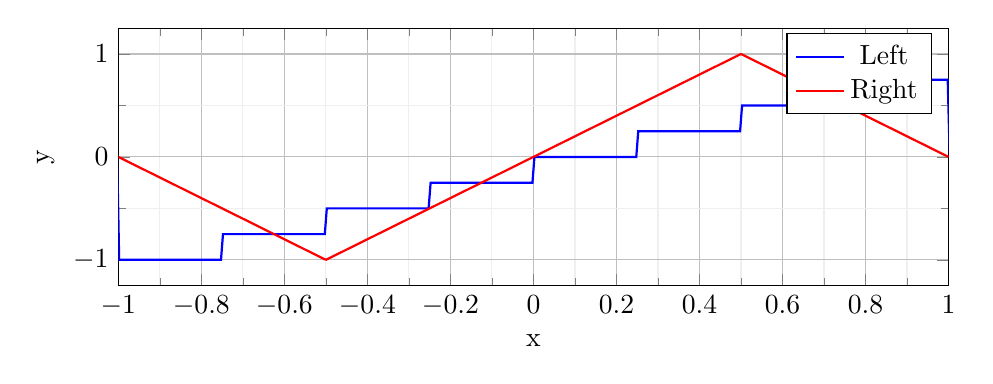
\begin{tikzpicture}
\begin{axis}[
    xmin = -1, xmax = 1,
    ymin = -1.25, ymax = 1.25,
    grid = both,
    minor tick num = 1,
    major grid style = {lightgray},
    minor grid style = {lightgray!25},
    width = \textwidth,
    height = 0.40\textwidth,
    xlabel = x,
    ylabel = y]

    \addplot[
        domain = -1.2:1.2,
        samples = 500,
        thick,
        blue,
        ] 
        {
        (x > -1)*(x < 1)*(floor(4*x)/4)
        };


    \addplot[
        domain = -1:1,
        samples = 500,
        thick,
        red,
        ] 
        {
        (x > -0.5)*(x < 0.5)*(2*x) + (x < -0.5)*(-2*x-2)   + (x > 0.5)*(-2*x+2)
        };
    \legend{
        Left,
        Right,
        }
\end{axis}
\end{tikzpicture}
\end{center}
\label{app_fig}
\caption{The function approximated by each of the 2 groups.}
\end{figure}

\clearpage
\section{Laboratory}
Below are the results from approximating the triangle function using trigonometric functions for different numbers of terms, and N = 10000:\\
\begin{figure}[h!]
\begin{center}
\begin{tikzpicture}
\begin{axis}[
    xmin = -1, xmax = 1,
    ymin = -1.2, ymax = 1.2,
    grid = both,
    minor tick num = 1,
    major grid style = {lightgray},
    minor grid style = {lightgray!25},
    width = 0.45\textwidth,
    height = 0.50\textwidth,
    xlabel = x,
    ylabel = y,
    scaled x ticks=false]

    \addplot[color=blue,
        ]
        table [col sep=space, x index = 0, y index=1]{./plot_data/chapter_4/triangle_lab_5_trig_approx.dat};

    \addplot[color=green,
        ]
        table [col sep=space, x index = 0, y index=2]{./plot_data/chapter_4/triangle_lab_5_trig_approx.dat};

    \addplot[color=red,
        ]
        table [col sep=space, x index = 0, y index=3]{./plot_data/chapter_4/triangle_lab_5_trig_approx.dat};

    \addplot[color=orange,
        ]
        table [col sep=space, x index = 0, y index=4]{./plot_data/chapter_4/triangle_lab_5_trig_approx.dat};

    \addplot[color=black,
        ]
        table [col sep=space, x index = 0, y index=5]{./plot_data/chapter_4/triangle_lab_5_trig_approx.dat};


    \addplot[color=purple,
        ]
        table [col sep=space, x index = 0, y index=6]{./plot_data/chapter_4/triangle_lab_5_trig_approx.dat};

    \legend{
        $S = 5$,
        $S = 10$,
        $S = 15$,
        $S = 20$,
        $S = 25$,
        $S = 30$}
\end{axis}
\end{tikzpicture}
\begin{tikzpicture}
\begin{axis}[
    xmin = -1, xmax = 1,
    ymin = -1.2, ymax = 1.2,
    grid = both,
    minor tick num = 1,
    major grid style = {lightgray},
    minor grid style = {lightgray!25},
    width = 0.45\textwidth,
    height = 0.5\textwidth,
    xlabel = x,
    ylabel = y,
    scaled x ticks=false]

    \addplot[color=blue,
        ]
        table [col sep=space, x index = 0, y index=1]{./plot_data/chapter_4/triangle_lab_5_trig_error.dat};

    \addplot[color=green,
        ]
        table [col sep=space, x index = 0, y index=2]{./plot_data/chapter_4/triangle_lab_5_trig_error.dat};

    \addplot[color=red,
        ]
        table [col sep=space, x index = 0, y index=3]{./plot_data/chapter_4/triangle_lab_5_trig_error.dat};

    \addplot[color=orange,
        ]
        table [col sep=space, x index = 0, y index=4]{./plot_data/chapter_4/triangle_lab_5_trig_error.dat};

    \addplot[color=black,
        ]
        table [col sep=space, x index = 0, y index=5]{./plot_data/chapter_4/triangle_lab_5_trig_error.dat};


    \addplot[color=purple,
        ]
        table [col sep=space, x index = 0, y index=6]{./plot_data/chapter_4/triangle_lab_5_trig_error.dat};

    \legend{
        $S = 5$,
        $S = 10$,
        $S = 15$,
        $S = 20$,
        $S = 25$,
        $S = 30$}
\end{axis}
\end{tikzpicture}
\caption{Approximations using trigonometric functions on the left, differences between those and the original function on the right}
\end{center}
\end{figure}
\\
These can then be compared with approximations based on Legendre's polynomials:
\begin{figure}[h!]
\begin{center}
\begin{tikzpicture}
\begin{axis}[
    xmin = -1, xmax = 1,
    ymin = -1.2, ymax = 1.2,
    grid = both,
    minor tick num = 1,
    major grid style = {lightgray},
    minor grid style = {lightgray!25},
    width = 0.45\textwidth,
    height = 0.5\textwidth,
    xlabel = x,
    ylabel = y,
    scaled x ticks=false]

    \addplot[color=blue,
        ]
        table [col sep=space, x index = 0, y index=1]{./plot_data/chapter_4/triangle_lab_5_leg_approx.dat};

    \addplot[color=green,
        ]
        table [col sep=space, x index = 0, y index=2]{./plot_data/chapter_4/triangle_lab_5_leg_approx.dat};

    \addplot[color=red,
        ]
        table [col sep=space, x index = 0, y index=3]{./plot_data/chapter_4/triangle_lab_5_leg_approx.dat};

    \addplot[color=orange,
        ]
        table [col sep=space, x index = 0, y index=4]{./plot_data/chapter_4/triangle_lab_5_leg_approx.dat};

    \addplot[color=black,
        ]
        table [col sep=space, x index = 0, y index=5]{./plot_data/chapter_4/triangle_lab_5_leg_approx.dat};


    \addplot[color=purple,
        ]
        table [col sep=space, x index = 0, y index=6]{./plot_data/chapter_4/triangle_lab_5_leg_approx.dat};

    \legend{
        $S = 5$,
        $S = 10$,
        $S = 15$,
        $S = 20$,
        $S = 25$,
        $S = 30$}
\end{axis}
\end{tikzpicture}
\begin{tikzpicture}
\begin{axis}[
    xmin = -1, xmax = 1,
    ymin = -1.2, ymax = 1.2,
    grid = both,
    minor tick num = 1,
    major grid style = {lightgray},
    minor grid style = {lightgray!25},
    width = 0.45\textwidth,
    height = 0.5\textwidth,
    xlabel = x,
    ylabel = y,
    scaled x ticks=false]

    \addplot[color=blue,
        ]
        table [col sep=space, x index = 0, y index=1]{./plot_data/chapter_4/triangle_lab_5_leg_error.dat};

    \addplot[color=green,
        ]
        table [col sep=space, x index = 0, y index=2]{./plot_data/chapter_4/triangle_lab_5_leg_error.dat};

    \addplot[color=red,
        ]
        table [col sep=space, x index = 0, y index=3]{./plot_data/chapter_4/triangle_lab_5_leg_error.dat};

    \addplot[color=orange,
        ]
        table [col sep=space, x index = 0, y index=4]{./plot_data/chapter_4/triangle_lab_5_leg_error.dat};

    \addplot[color=black,
        ]
        table [col sep=space, x index = 0, y index=5]{./plot_data/chapter_4/triangle_lab_5_leg_error.dat};


    \addplot[color=purple,
        ]
        table [col sep=space, x index = 0, y index=6]{./plot_data/chapter_4/triangle_lab_5_leg_error.dat};

    \legend{
        $S = 5$,
        $S = 10$,
        $S = 15$,
        $S = 20$,
        $S = 25$,
        $S = 30$}
\end{axis}

    
\end{tikzpicture}

\caption{Approximations using Legendre's polynomials on the left, differences between those and the original function on the right}
\end{center}
\end{figure}
\clearpage
The triangle function is well approximated with both bases. However, since both of these bases are composed of functions which are differentiable over the whole approximation domain, they struggle with approximating the non-differentiable points of the original function.\\
To compare both of these bases, we can look at the $L_2$ norm of their approximation error as a function of S:
%%

\begin{figure}[h!]
\begin{center}
\begin{tikzpicture}
\begin{axis}[
    xmin = 5, xmax = 30,
    ymin = 0, ymax = 5,
    grid = both,
    minor tick num = 1,
    major grid style = {lightgray},
    minor grid style = {lightgray!25},
    width = \textwidth,
    height = 0.5\textwidth,
    xlabel = S,
    ylabel = $\norm{\cdot}_2$,
    scaled x ticks=false]


    \addplot[color=blue,
        ]
        table [col sep=space, x index = 0, y index=1]{./plot_data/chapter_4/lab_5_trig_norms.dat};
    \addplot[color=red,
        ]
        table [col sep=space, x index = 0, y index=2]{./plot_data/chapter_4/lab_5_trig_norms.dat};
    \legend{
        Trigonometric functions,
        Legendre Polynomials}
\end{axis}

    
\end{tikzpicture}

\caption{$L_2$ norm of the error as a function of S for N = 10000}
\end{center}
\end{figure}

The above plot shows, that both bases are comparable, with the Legendre polynomials performing a little worse.\\
\clearpage
This then poses a question, why would one consider using these polynomials as a basis? In an attempt to try and answer this question, the floor function from the left group will be approximated:

\begin{figure}[h!]
\begin{center}
\begin{tikzpicture}
\begin{axis}[
    xmin = -1, xmax = 1,
    ymin = -1.2, ymax = 1.2,
    grid = both,
    minor tick num = 1,
    major grid style = {lightgray},
    minor grid style = {lightgray!25},
    width = 0.45\textwidth,
    height = 0.45\textwidth,
    xlabel = x,
    ylabel = y,
    scaled x ticks=false]

    \addplot[color=blue,
        ]
        table [col sep=space, x index = 0, y index=1]{./plot_data/chapter_4/step_lab_5_trig_approx.dat};

    \addplot[color=green,
        ]
        table [col sep=space, x index = 0, y index=2]{./plot_data/chapter_4/step_lab_5_trig_approx.dat};

    \addplot[color=red,
        ]
        table [col sep=space, x index = 0, y index=3]{./plot_data/chapter_4/step_lab_5_trig_approx.dat};

    \addplot[color=orange,
        ]
        table [col sep=space, x index = 0, y index=4]{./plot_data/chapter_4/step_lab_5_trig_approx.dat};




    \legend{
        $S = 5$,
        $S = 10$,
        $S = 20$,
        $S = 35$}
\end{axis}
\end{tikzpicture}
\begin{tikzpicture}
\begin{axis}[
    xmin = -1, xmax = 1,
    ymin = -1.2, ymax = 1.2,
    grid = both,
    minor tick num = 1,
    major grid style = {lightgray},
    minor grid style = {lightgray!25},
    width = 0.45\textwidth,
    height = 0.45\textwidth,
    xlabel = x,
    ylabel = y,
    scaled x ticks=false]

    \addplot[color=blue,
        ]
        table [col sep=space, x index = 0, y index=1]{./plot_data/chapter_4/step_lab_5_trig_error.dat};

    \addplot[color=green,
        ]
        table [col sep=space, x index = 0, y index=2]{./plot_data/chapter_4/step_lab_5_trig_error.dat};

    \addplot[color=red,
        ]
        table [col sep=space, x index = 0, y index=3]{./plot_data/chapter_4/step_lab_5_trig_error.dat};

    \addplot[color=orange,
        ]
        table [col sep=space, x index = 0, y index=4]{./plot_data/chapter_4/step_lab_5_trig_error.dat};




    \legend{
        $S = 5$,
        $S = 10$,
        $S = 20$,
        $S = 35$}
\end{axis}

    
\end{tikzpicture}

\caption{Approximations using trigonometric functions on the left, differences between those and the original function on the right}
\end{center}
\end{figure}
\\
These can then be compared with approximations based on Legendre's polynomials:
\\
\begin{figure}[h!]
\begin{center}
\begin{tikzpicture}
\begin{axis}[
    xmin = -1, xmax = 1,
    ymin = -1.2, ymax = 1.2,
    grid = both,
    minor tick num = 1,
    major grid style = {lightgray},
    minor grid style = {lightgray!25},
    width = 0.45\textwidth,
    height = 0.45\textwidth,
    xlabel = x,
    ylabel = y,
    scaled x ticks=false]

    \addplot[color=blue,
        ]
        table [col sep=space, x index = 0, y index=1]{./plot_data/chapter_4/step_lab_5_leg_approx.dat};

    \addplot[color=green,
        ]
        table [col sep=space, x index = 0, y index=2]{./plot_data/chapter_4/step_lab_5_leg_approx.dat};

    \addplot[color=red,
        ]
        table [col sep=space, x index = 0, y index=3]{./plot_data/chapter_4/step_lab_5_leg_approx.dat};

    \addplot[color=orange,
        ]
        table [col sep=space, x index = 0, y index=4]{./plot_data/chapter_4/step_lab_5_leg_approx.dat};


    \legend{
        $S = 5$,
        $S = 10$,
       $S = 20$,
        $S = 35$}
\end{axis}
\end{tikzpicture}
\begin{tikzpicture}
\begin{axis}[
    xmin = -1, xmax = 1,
    ymin = -1.2, ymax = 1.2,
    grid = both,
    minor tick num = 1,
    major grid style = {lightgray},
    minor grid style = {lightgray!25},
    width = 0.45\textwidth,
    height = 0.45\textwidth,
    xlabel = x,
    ylabel = y,
    scaled x ticks=false]

    \addplot[color=blue,
        ]
        table [col sep=space, x index = 0, y index=1]{./plot_data/chapter_4/step_lab_5_leg_error.dat};

    \addplot[color=green,
        ]
        table [col sep=space, x index = 0, y index=2]{./plot_data/chapter_4/step_lab_5_leg_error.dat};

    \addplot[color=red,
        ]
        table [col sep=space, x index = 0, y index=3]{./plot_data/chapter_4/step_lab_5_leg_error.dat};

    \addplot[color=orange,
        ]
        table [col sep=space, x index = 0, y index=4]{./plot_data/chapter_4/step_lab_5_leg_error.dat};




    \legend{
        $S = 5$,
        $S = 10$,
        $S = 20$,
        $S = 35$,
        }
\end{axis}

    
\end{tikzpicture}

\caption{Approximations using Legendre's polynomials on the left, differences between those and the original function on the right}
\end{center}
\end{figure}

\clearpage
The step function is well approximated with both bases. However, since both of these functions are differentiable over the whole approximation domain, they struggle the most with approximating the non-differentiable points of the original function.\\
To compare both of these bases, we can look at the $L_2$ norm of their approximation error as a function of S:
%%
\\
\begin{figure}[h!]
\begin{center}
\begin{tikzpicture}
\begin{axis}[
    xmin = 5, xmax = 35,
    ymin = 0, ymax = 15,
    grid = both,
    minor tick num = 1,
    major grid style = {lightgray},
    minor grid style = {lightgray!25},
    width = \textwidth,
    height = 0.5\textwidth,
    xlabel = S,
    ylabel = $\norm{\cdot}_2$,
    scaled x ticks=false]


    \addplot[color=blue,
        ]
        table [col sep=space, x index = 0, y index=1]{./plot_data/chapter_4/lab_5_step_norms.dat};
    \addplot[color=red,
        ]
        table [col sep=space, x index = 0, y index=2]{./plot_data/chapter_4/lab_5_step_norms.dat};
    \legend{
        Trigonometric functions,
        Legendre Polynomials}
\end{axis}
\end{tikzpicture}
\caption{$L_2$ norm of the error as a function of S for N = 10000}
\end{center}
\end{figure}
\\
From the above it can be surmised, that for functions with discontinuities,or at least ones which change their values very quickly, Legendre polynomials perform better than ordinary trigonometric functions. Another advantage Legendre polynomials have over trigonometric function is better performance at the boundary points. Trigonometric functions suffer from large errors at the boundary, which doesn't seem to be the case for Legendre polynomials. This difficulty with handling non-zero values at the boundary probably accounts for most of the error.





\section{Conclusions}
For certain functions these rational approximations work very well, for others not so much. Both of the analysed bases struggle to accurately describe points where the original function is either discontinuous, or non-differentiable. Judging however by their performance with the floor function, is appears that Legendre's polynomials are a better basis for approximating discontinuous functions.

